\chapter{Resultados}
\label{chap:resultados}

El resultado más tangible de este proyecto es la aplicación móvil desarrollada. Sin embargo, y pese a ser el mas visible, no es el único. Detrás de esta aplicación hay un sistema que le da soporte y permite que sea más que un mero cascarón, entre ellos, el sistema de comunicación, el de gestión de imágenes y más importante el de recomendación. Se ha desarrollado un sistema capaz de comunicar a varios usuarios a través de mensajes e imágenes, capaz de realizar búsquedas de estas imágenes y capaz de adaptar las imágenes proporcionadas por esta búsqueda a cada usuario de la aplicación.

De esta manera, cuando cualquier usuario comienza a realizar las primeras consultas y recibe las primeras recomendaciones, todas son iguales. Conforme avance la utilización de la aplicación por parte del usuario, esta se irá adaptando a este y recomendándole aquellas imágenes que más se adecuen a sus gustos. Pongamos por caso que el usuario al que llamaremos \textit{Usuario1} es muy aficionado de las imágenes ilustradas o dibujos. Conforme este continúe seleccionando estas imágenes, el sistema al analizarlas mediante la \ac{API} Cloud Visión, detectará que estas imágenes son de este tipo y las etiquetará como tal. Además, si otros usuarios que también gustan de seleccionar estas imágenes han seleccionado la misma, se establecerá relación entre ellos. Si continúan seleccionando imágenes similares, su relación se incrementará, lo cuál afectará posteriormente en la recomendación. Por otro lado, si se detecta que estas imágenes proceden de un sitio web concreto que esta especializado en imágenes del tipo ilustración, este tipo de imágenes también serán recomendadas por el algoritmo basado en contenido. Este comportamiento se puede trasladar a otros entornos, como por ejemplo imágenes en las que haya muchos colores, o imágenes en blanco y negro. En la Figura \ref{fig:progreso-recomendacion} se puede ver un ejemplo de este progreso.

\begin{figure}[!h]
\begin{center}
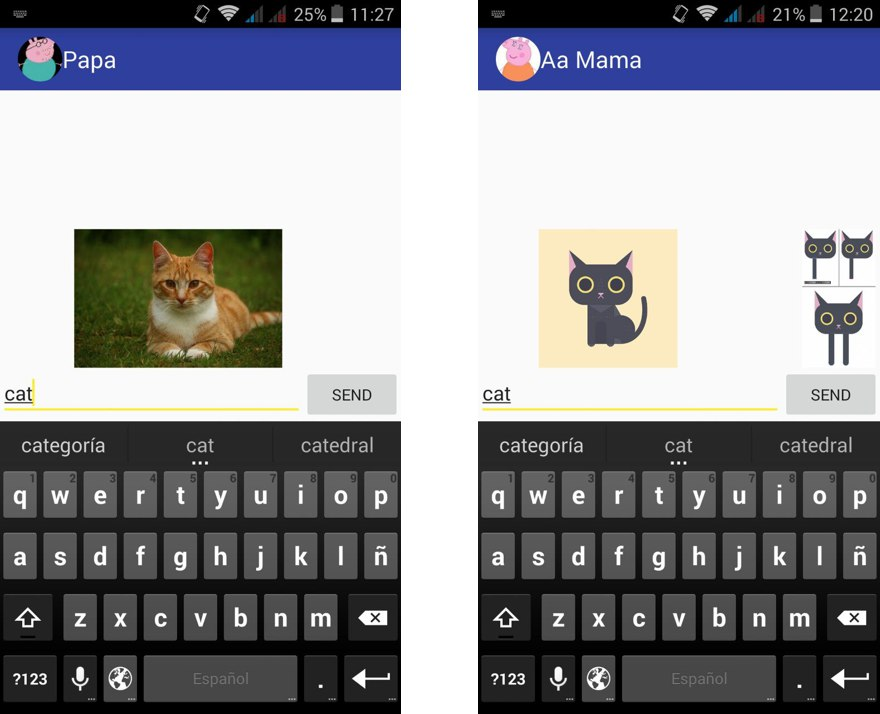
\includegraphics[width=1.1\textwidth]{./figures/progreso-recomendacion.jpg}
\caption{Progreso-recomendacion}
\label{fig:progreso-recomendacion}
\end{center}
\end{figure}

Todo este aprendizaje y adaptación al usuario dependen en gran medida de la técnica colaborativa, especialmente cuando se refiere a largo plazo. Esto es así, porque en última instancia, lo que mejor se puede recomendar a un usuario es aquello que se sabe que le va a interesar, y para ello lo más fácil es observar si le ha gustado a sus vecinos, o en otras palabras, a los usuarios más afines a este. Sin embargo, y debido a las limitaciones y carácter de este proyecto ha sido imposible realizar un estudio de los resultados con los usuarios suficientes como para establecer el verdadero potencial de este sistema, dejando esta tarea para futuros trabajos como se verá en el siguiente capítulo.